\section{Evaluation}\label{eva}
% In this section, we implement \NAME
% and thoroughly evaluate its efficiency. 
Throughout the experiments,
we wish to answer the following two main research questions (RQs).
\begin{itemize}
    \item {\bf{RQ1}}: How efficient are the individual components of \NAME
    compare to state-of-the-art (SOTA) methods? (\cref{sec:qual_comp}, \cref{eva: microbenchmarks}) 
    \item {\bf{RQ2}}: How does the performance of \NAME in specific SQL queries 
    and end-to-end data analysis benchmark compare to other methods? 
    (\cref{eva: sql_benchmark})
\end{itemize}
%We note in the first question, we want to benchmark

\subsection{Experiment Setup}\label{eva:Arch}
The entire \NAME is implemented using C++17 and 
compiled with GCC 10.3.0 based on Microsoft SEAL~\cite{codeseal},
%(an easy-to-use open-source homomorphic encryption library)
OpenPEGASUS~\cite{codepegasus}, and TFHEpp~\cite{codetfhepp}.
% , which are the state-of-the-art implementations
% of the CKKS and TFHE schemes.
For single-core microbenchmarks, the experiments are  carried out on 
an Intel Xeon Gold 6226R processor with 512GB of RAM. Meanwhile,
the experiments for the TPC-H benchmarks~\cite{tpc_h} reported in \cref{eva: sql_benchmark} are performed
on two servers with a total of four Intel Xeon Gold 5318Y processors with
96 cores and 1TB of RAM.
%\textbf{Instantiated Parameters}: 
The instantiated parameters are outlined in \cref{tab:parameters}, which provide 
at least 128-bit of security level according to~\cite{lweestimator}.
We fix the standard deviation 
$\sigma$ of the 
noise distribution $\chi$ and set the security level $\lambda$ 
to meet the Homomorphic Encryption Standard~\cite{HomomorphicEncryptionSecurityStandard}. 
It is noted that we actually achieved better security than the most relevant work HEDA,
as HEDA only guarantees an 80-bit security~\cite{heda}.

% Here, 
% we take $\sigma = 3.19 
% \approx 8/\sqrt{2\pi } $ and the resulting $\lambda = 128$-bit.




\subsection{Qualitative Assessments for $\homcomp$}\label{sec:qual_comp}
\begin{table}[t!] 
    \centering
    \caption{Benchmark Results for Homomorphic $\geq$}
    % \vspace{0em}
        \begin{tabular}{cccccc}
            \toprule
            Precision & Methods & \multicolumn{2}{c}{Latency (ms)} & \multicolumn{2}{c}{Ciphertext (kB)} \\
                 %&         & (ms)      &         & (kB) & \\
            \midrule
             \multirow{4}*{4} & PEGASUS~\cite{pegasus} & 681 & $37.83\times$ & 8 & $2\times$ \\
             & SortingHat~\cite{sortinghat} & 444 & $24.67\times$ & 10 & $2.5\times$ \\
             & Liu \etal ~\cite{largeprecision} & 2040 & $113\times$ & 16 & $4\times$ \\
             % & Antonio\cite{revisiting} & 70 & $3.89\times$ & 5 & $1.25\times$ \\
             & \textbf{Ours} & 18 & $1\times$ & 4 & $1\times$ \\
             \midrule
            % \midrule
            %  \multirow{4}*{8} & Pegasus~\cite{pegasus} & 3027& $56.06\times$ & 8 & $2\times$ \\
            %  & SortingHat~\cite{sortinghat} & 1030 & $19.07\times$ & 19 & $4.75\times$ \\
            %  & Liu~\cite{largeprecision} & 4439 & $82.2\times$ & 16 & $4\times$ \\
            %  % & Antonio\cite{revisiting} & 138 & $2.56\times$ & 10 & $2.5\times$ \\
            %  & \NAME & \textbf{54} & $1\times$ & \textbf{4} & $1\times$ \\
            % \midrule
             \multirow{4}*{16} & PEGASUS~\cite{pegasus} & --- & --- & --- & --- \\
             & SortingHat~\cite{sortinghat} & 2186 & $8.13\times$ & 38 & $2.38\times$ \\
             & Liu \etal~\cite{largeprecision} & 7992 & $29.71\times$ & 16 & $1\times$ \\
             % & Antonio\cite{revisiting} & 277 & $1.03\times$ & 20 & $1.25\times$ \\
             & \textbf{Ours}  & 269 & $1\times$ & 16 & $1\times$ \\
            \midrule
             \multirow{4}*{32} & PEGASUS~\cite{pegasus} & --- & --- & --- & --- \\
             & SortingHat~\cite{sortinghat} & 4329 & $7.67\times$ & 76 & $4.75\times$ \\
             & Liu \etal~\cite{largeprecision} & --- & --- & --- & ---\\
             % & Antonio\cite{revisiting} & 202 & $1.22\times$ & 40 & $2.5\times$ \\
             & \textbf{Ours}  & 564 & $1\times$ & 16 & $1\times$ \\
            \bottomrule
        \end{tabular}
    \label{tab:combenchmark}
    {\footnotesize{$-$ means
    the method does not support such bits of precision.}}
    % \vspace{-3mm}
\end{table}

\begin{figure*}[t!]
   \begin{center}
    \begin{subfigure}[b]{0.3\textwidth}
    \centering
    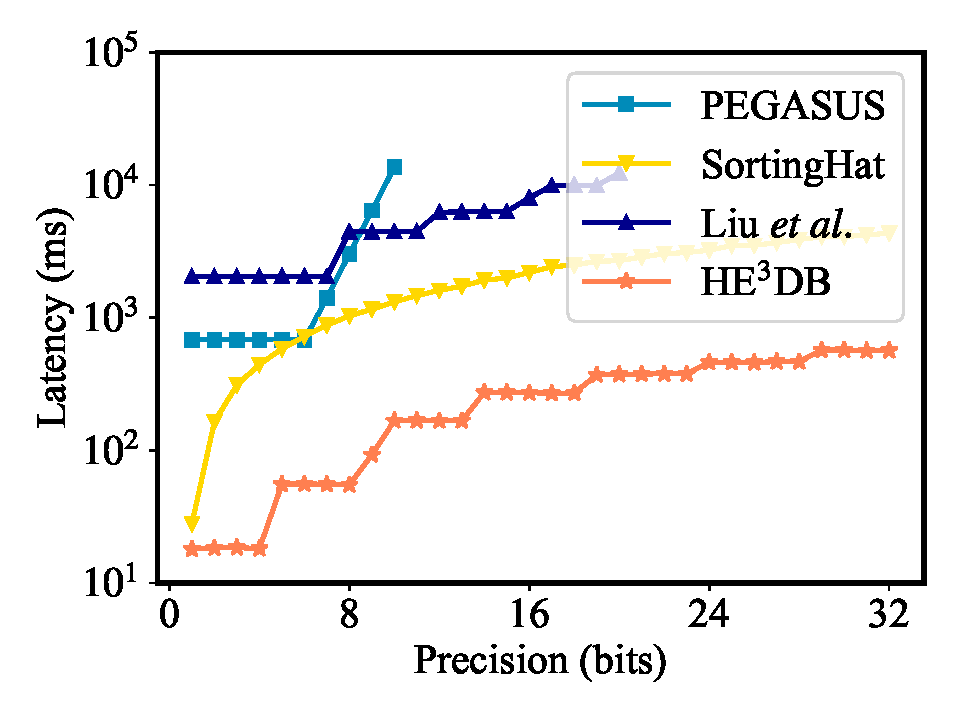
\includegraphics[width=\linewidth]{figure/com_micro_geq.pdf}
    % \vspace{-2em}
    \caption{Homomorphic $\geq$}
    \label{fig:homcompbench1}
    \end{subfigure}%
    \hfill
    \begin{subfigure}[b]{0.3\textwidth}
    \centering
    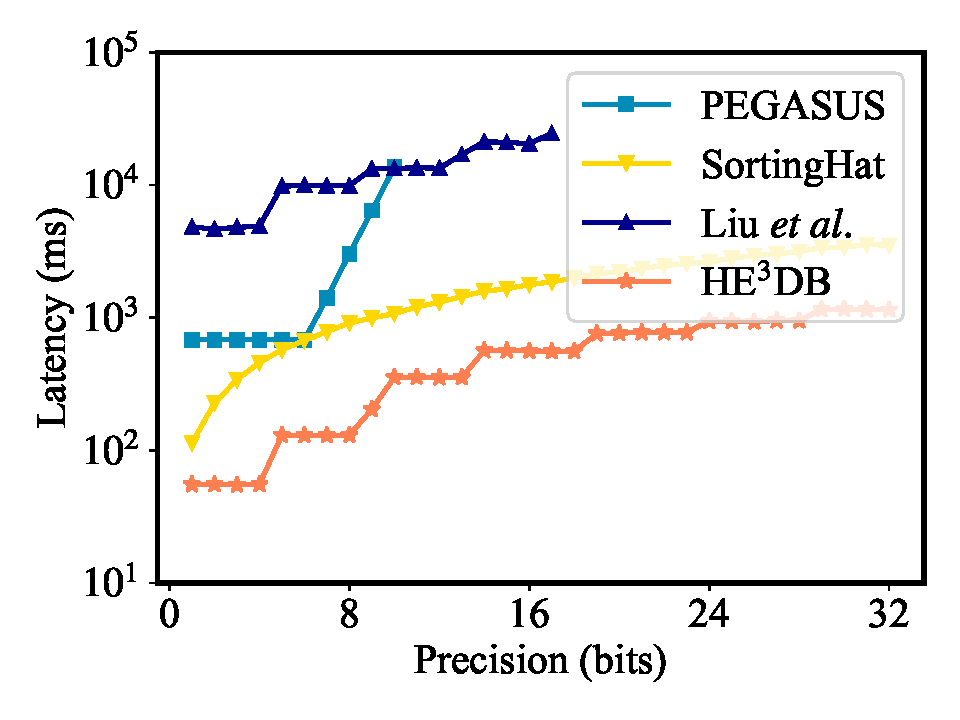
\includegraphics[width=\linewidth]{figure/com_micro_eq.pdf}
    % \vspace{-2em}
    \caption{Homomorphic $==$}
    \label{fig:homcompbench2}
    \end{subfigure}%
    \hfill
    \begin{subfigure}[b]{0.3\textwidth}
    \centering
    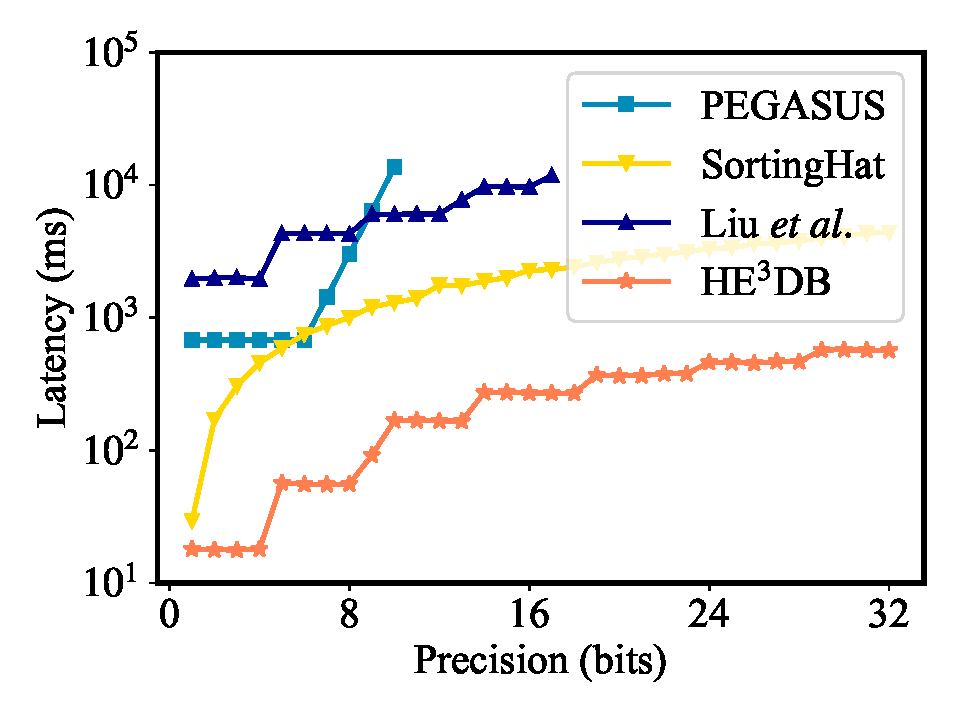
\includegraphics[width=\linewidth]{figure/com_micro_g.pdf}
    % \vspace{-2em}
    \caption{Homomorphic $>$}
    \label{fig:homcompbench3}
    \end{subfigure}%
   
   \end{center}
    % \vspace{-0.5em}
      \caption{Benchmark results for homomorphic comparison for the 
      $\geq, ==, >$ comparison operators 
       with varying bit precision.}
       \Description{Benchmark results for homomorphic comparison for the 
      $\geq, ==, >$ comparison operators 
       with varying bit precision. 
       The horizontal axis is the bits of precision, and the vertical axis is the latency. 
       Our results achieve competitive performance across different
       comparison operators}
   \label{fig: homcompbench}
   % \vspace{-0.5em}
\end{figure*}
Since $\homcomp$ is one of the key homomorphic operators proposed
in this work, we first compare our $\homcomp$ with other related 
homomorphic comparison algorithms qualitatively, and
defer quantitative results to \cref{eva: microbenchmarks}.
% have their own advantages and 
% method selection depends on the application.
In the beginning, we note that approaches like PEGASUS~\cite{pegasus} and the method 
proposed by Liu \etal~\cite{largeprecision} focus on evaluating
arbitrary logic
functions over homomorphically encrypted ciphertext,
%by proposing efficient or large-precision PBS algorithms
while \NAME concentrates on the design of a homomorphic comparison algorithm.
Therefore, our method achieves better comparison accuracy as well
as efficiency than~\cite{pegasus, largeprecision}. In contrast
to general methods, 
SortingHat~\cite{sortinghat} proposes an efficient plaintext-ciphertext 
comparison algorithm, where one of the inputs to the comparison
is known to the server. Nonetheless, under an SDO setting,
SortingHat shows poor efficiency for ciphertext-ciphertext
comparisons. The method of Antonio \etal~\cite{revisiting} 
encrypts the input in a bit-wise manner, where binary circuits
can be used to construct fast and high-precision
homomorphic comparison. However, due to the encoding scheme, 
the algorithm in~\cite{revisiting} produces
a comparison result of $\{-1,0,1\}$, which cannot be used as
filters for subsequent aggregations.
Similarly, the polynomial approximation technique proposed by 
Cheon \etal~\cite{ckkscomparison} cannot support encrypted 
aggregations over results from equality tests \texttt{==}, for the approximate polynomial evaluates
to $1/2$ when the inputs are equal.
On the other hand, some works also suggest to encrypt all database items bit-by-bit in a
SIMD manner to accelerate the comparison process~\cite{aphadb, khedr2015shield}.
%due to the noise growth of RLWE ciphertext 
%as we discussed in \cref{pre:he_type}.
However, in such approaches, the client encrypts the 
entire database using an {\it{a-priori}} fixed-set parameters 
that are dependent on
the pre-defined maximum predicate depth. As a result,
any query that requires more predicate evaluations than the
pre-defined maximum depth cannot be directly
evaluated. Here, the only solution is to re-encrypt
entire database using a new set of encryption parameters, which
can be too costly for SDO clients.
%respectively representing the \texttt{<}, \texttt{==} and \texttt{>}.
% However, Antonio's approach~\cite{revisiting} does not support 
% the encrypted database scenarios as the result of the comparison 
% could not perform logic gate operation between various predicates.

% Different from the above approaches, a line of works investigate
% how to utilize polynomial approximations 
% to evaluate homomorphic comparisons over RLWE 
% ciphertexts~\cite{ckkscomparison}. 
% By leveraging
% the SIMD capability of RLWE ciphertext,
% such algorithm can achieve fast evaluation speed when processing
% a large number of parallel comparisons.
% Nonetheless, both of their methods do not meet the elasticity requirement.


% However, changing encryption parameters in~\cite{aphadb} requires the re-encryption
% of the entire database, which can bring about severe communcation 
% burdens on the client side in practice.
% encrypted queries that are more complicated than such depth.
% We list the qualitative comparisons between existing methods and 
% provide quantitative comparisons in \cref{eva: microbenchmarks}.

% Since not all of the methods summarized
% in \cref{eva: microbenchmarks} have the same design objective,

\subsection{Evaluating Cryptographic Building Blocks}\label{eva: microbenchmarks}

\begin{figure*}[t!]
    \begin{minipage}[t]{0.5\linewidth}
    \centering
    \begin{subfigure}[b]{0.5\textwidth}
    \centering
    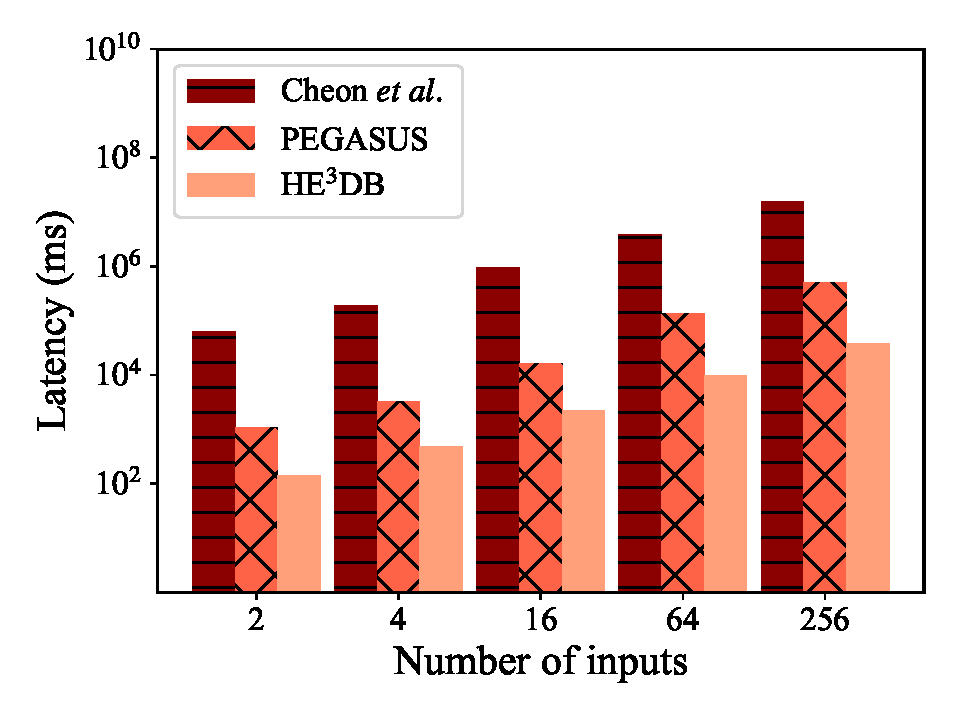
\includegraphics[width=\linewidth]{figure/minbench_4.pdf}
    % \vspace{-2em}
    \caption{4-bit $\dbmin$}
    \label{fig:homminbench4}
    \end{subfigure}%
    \hfill
    \begin{subfigure}[b]{0.5\textwidth}
    \centering
    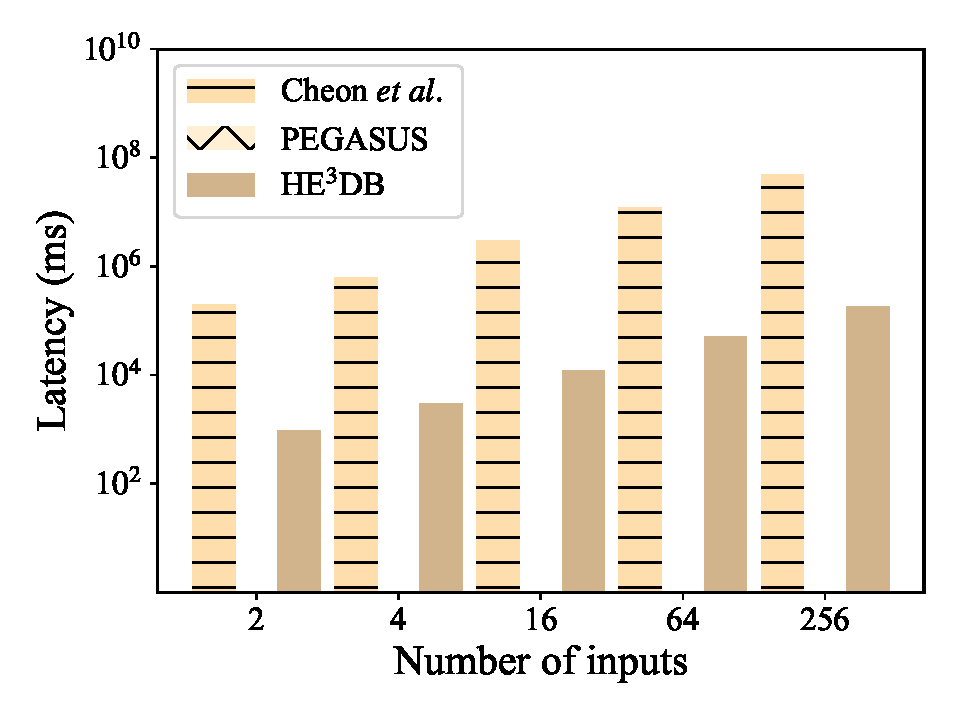
\includegraphics[width=\linewidth]{figure/minbench_16.pdf}
    % \vspace{-2em}
    \caption{16-bit $\dbmin$}
    \label{fig:homminbench16}
    \end{subfigure}%
    \caption{Benchmark results for Homomorphic $\dbmin$.}
    \Description{Benchmark results for Homomorphic $\dbmin$. The horizontal axis is the number of inputs, and the vertical axis is the latency. From the result, our performance is on average 
    around one order of magnitude faster than PEGASUS~\cite{pegasus}
    and two orders of magnitude faster than ~\cite{ckkscomparison}.}
    \label{fig: homminbench}
    \end{minipage}%
    \begin{minipage}[t]{0.5\linewidth}
    \centering
    \begin{subfigure}[b]{0.5\textwidth}
    \centering
    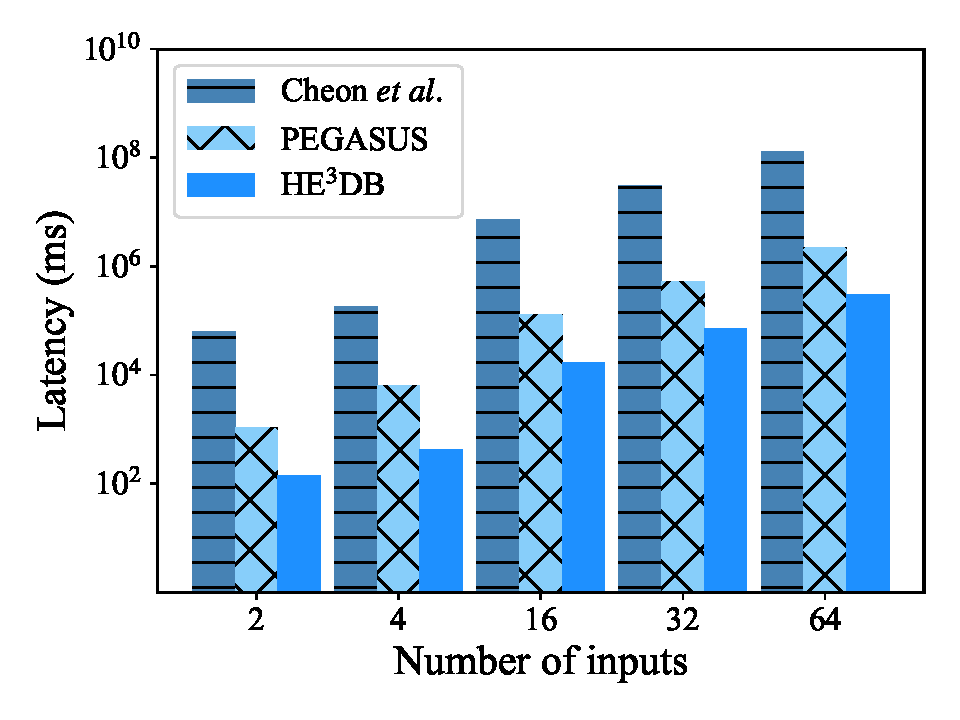
\includegraphics[width=\linewidth]{figure/sortbench_4.pdf}
    % \vspace{-2em}
    \caption{4-bit \orderby}
    \label{fig:homsortbench4}
    \end{subfigure}%
    \hfill
    \begin{subfigure}[b]{0.5\textwidth}
    \centering
    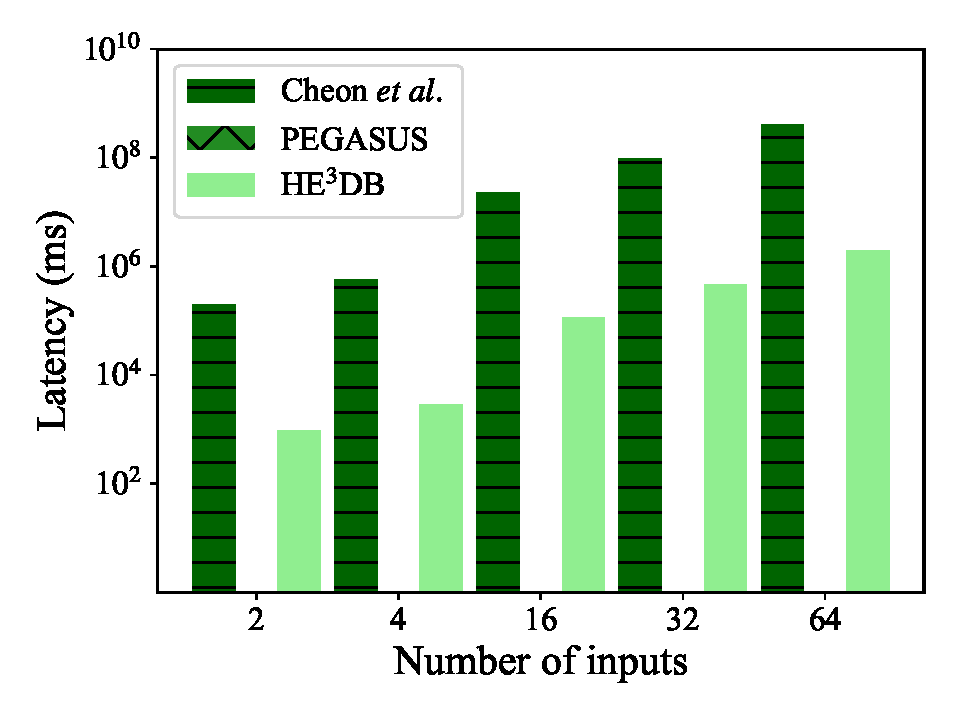
\includegraphics[width=\linewidth]{figure/sortbench_16.pdf}
    % \vspace{-2em}
    \caption{16-bit \orderby}
    \label{fig:homsortbench16}
    \end{subfigure}%
    \caption{Benchmark results for Homomorphic $\orderby$.}
    \Description{Benchmark results for Homomorphic $\orderby$. The horizontal axis is the number of inputs, and the vertical axis is the latency. From the results, our performance is on average 
    around one order of magnitude faster than PEGASUS~\cite{pegasus}
    and two orders of magnitude faster than ~\cite{ckkscomparison}.}
    \label{fig: homsortbench}
    \end{minipage}
   % \begin{center}
   %  \begin{subfigure}[b]{0.25\textwidth}
   %  \centering
   %  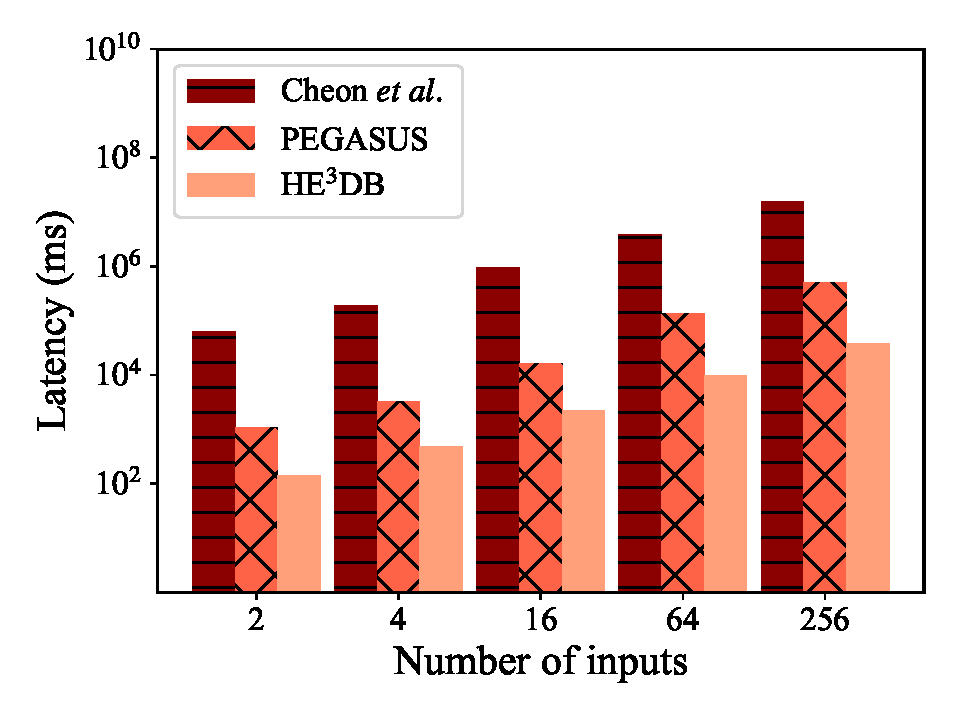
\includegraphics[width=\linewidth]{figure/minbench_4.pdf}
   %  % \vspace{-2em}
   %  \caption{4-bit}
   %  \label{fig:homminbench4}
   %  \end{subfigure}%
   %  \hfill
   %  \begin{subfigure}[b]{0.25\textwidth}
   %  \centering
   %  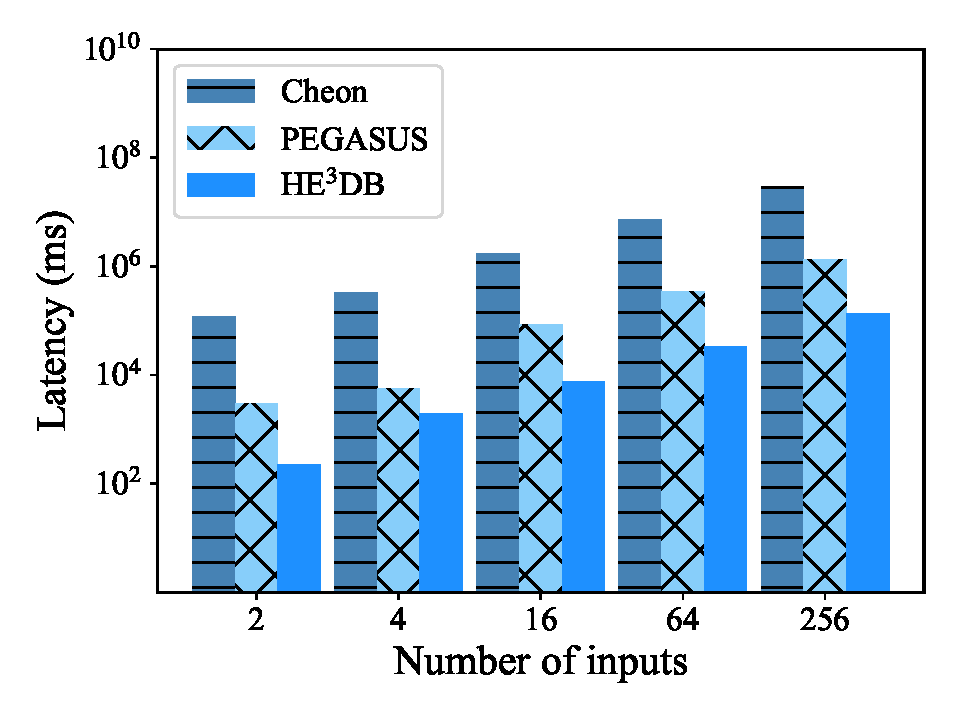
\includegraphics[width=\linewidth]{figure/minbench_8.pdf}
   %  % \vspace{-2em}
   %  \caption{8-bit}
   %  \label{fig:homminbench8}
   %  \end{subfigure}%
   %  \hfill
   %  \begin{subfigure}[b]{0.25\textwidth}
   %  \centering
   %  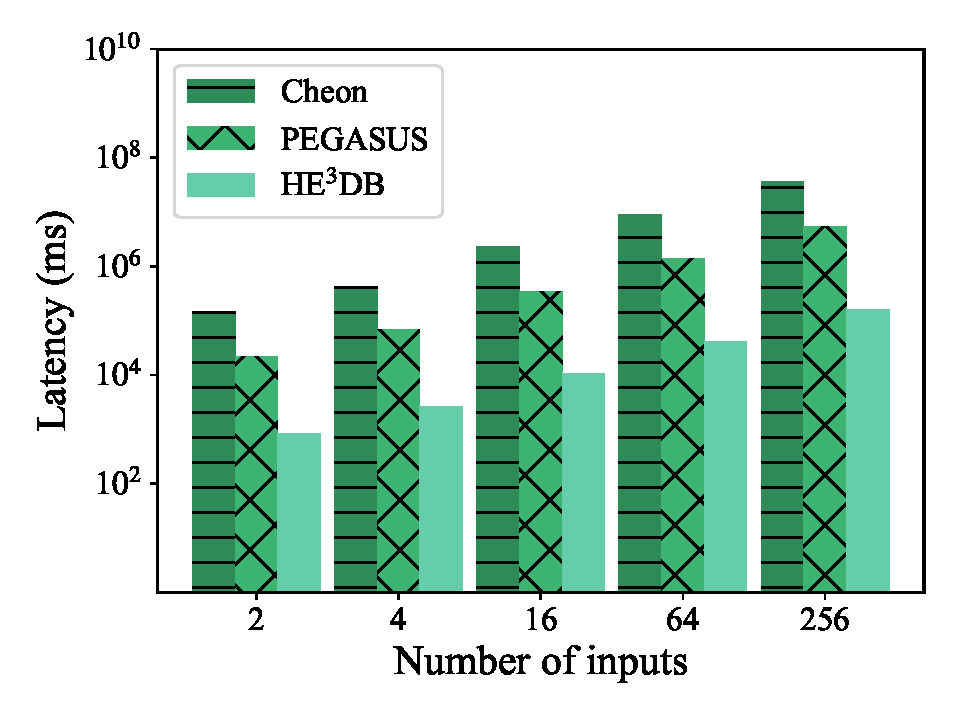
\includegraphics[width=\linewidth]{figure/minbench_12.pdf}
   %  % \vspace{-2em}
   %  \caption{12-bit}
   %  \label{fig:homminbench12}
   %  \end{subfigure}%
   %  \hfill
   %  \begin{subfigure}[b]{0.25\textwidth}
   %  \centering
   %  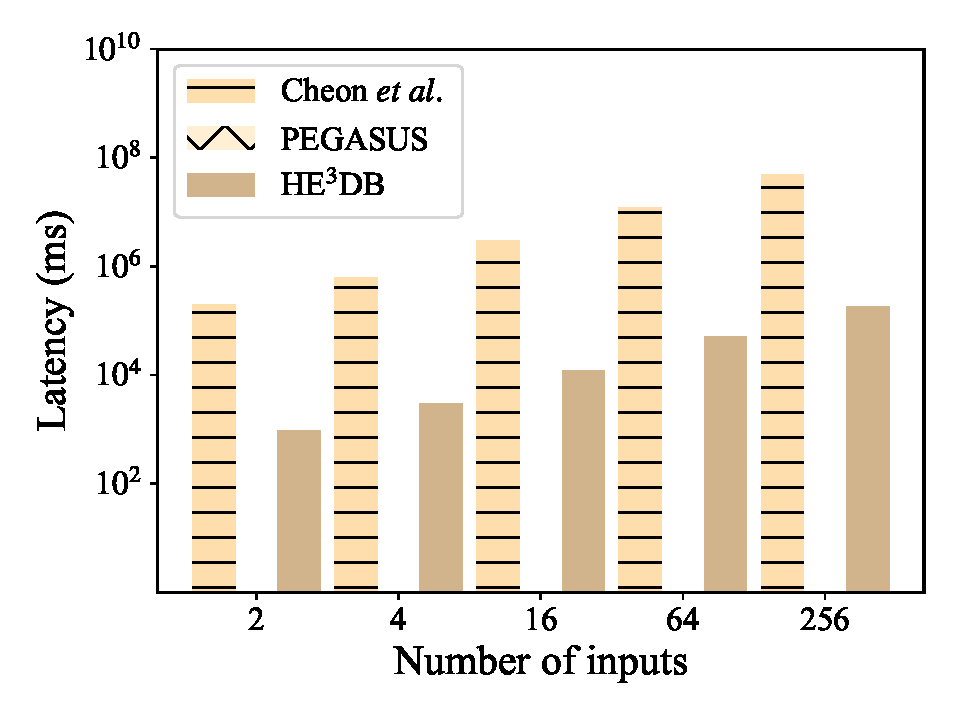
\includegraphics[width=\linewidth]{figure/minbench_16.pdf}
   %  % \vspace{-2em}
   %  \caption{16-bit}
   %  \label{fig:homminbench16}
   %  \end{subfigure}%
   
   % \end{center}
   %  % \vspace{-0.5em}
   %    \caption{Homomorphic MIN benchmark between $2,4,16,64,256$ numbers
   %          with $4,8,12$, and $16$ bits of precision.} 
   % \label{fig: homminbench}
   % \vspace{-0.5em}
\end{figure*}


%Here, we answer {\bf{RQ1}}. 
To answer {\bf{RQ1}}, we benchmark the efficiency of each of the 
cryptographic building blocks proposed in \cref{block},
including homomorphic comparison in \cref{block: comparison}, 
homomorphic \texttt{MIX/MAX} evaluation in \cref{block: minmax}
and ciphertext conversion in \cref{block: LWEsPack}. 
% The results
% are summarized as follows.

% {\bf{Homomorphic comparison}}:
%\subsubsection{Homomorphic comparison}
First of all, we compare the proposed $\homcomp$ with the best known 
existing works that support unbounded-depth predicate
evaluation, and the results are summarized in \cref{tab:combenchmark}.
We re-implement some of the existing works based on their open-source 
implementations~\cite{codepegasus, codesortinghat, codeopenfhe}
to fit our purpose (i.e., ciphertext-ciphertext comparison).
As observed in \cref{tab:combenchmark}, we are 7$\times$--113$\times$
faster than existing methods. Meanwhile, we can reduce the ciphertext
size by as much as 4.75$\times$ owing to our elastic ciphertext 
management policy.
% In addition,
% In \cref{tab:combenchmark}, we sketch the change
% of latency and ciphertext size on the predicate comparison operator $\geq$ 
% indifferent bits of precision.
% Specifically, in terms of latency, we achieve
% $24.67\times$, $19.07\times$, $8.13\times$ and $7.67\times$
% faster than the second best results on $4,8,12$, and $16$ bits of 
% precision, respectively.
In addition, as we can see from \cref{fig: homcompbench}, our
speedups are consistent across different comparison operators.
% shows the change of latency with 
% the increasing bits of precision for different methods. 
% As can be seen, our \NAME achieves lower latency
% compared to other methods on comparison operators $\geq, ==, >$, 
% which indicates higher efficiency.



%\subsubsection{Homomorphic \texttt{MIN/MAX}}
% {\bf{Homomorphic \dbmin/\dbmax}}: 
%\subsubsection{Homomorphic $\dbmin$/$\dbmax$ and $\orderby$}
Next, we compare the latency performance of the proposed homomorphic
\texttt{MIN/MAX} algorithms and SQL $\orderby$ operator to 
PEGASUS~\cite{pegasus} and Cheon \etal~\cite{ckkscomparison}
% and \NAME on the
% same numbers with the same bits of precision.
with a varying number of inputs and bit precision for the inputs.
As depicted in \cref{fig: homminbench} and \cref{fig: homsortbench},
our performance is on average around 
one order of magnitude faster than PEGASUS~\cite{pegasus},
and two orders of magnitude faster
than~\cite{ckkscomparison}.
Note in \cref{fig: homminbench} (b) and \cref{fig: homsortbench} (b) the 
histograms of PEGASUS~\cite{pegasus}
are left blank, for PEGASUS cannot support homomorphic \texttt{MIN/MAX} 
and $\orderby$ functions
over 16-bit operands.

%\subsubsection{Homomorphic ciphertext conversion}
% {\bf{Homomorphic Conversion}}: 
%\subsubsection{Homomorphic conversion}
% In ~\cref{tab:conversionbenchmark}, 
Lastly, to test the performance of the proposed $\repack$ operator, we
compare our algorithm to PEGASUS~\cite{pegasus} and 
Chen \etal~\cite{conversionhaochen}
over the task of converting $2^{15}$ LWE ciphertexts into
one RLWE ciphertext. Although PEGASUS~\cite{pegasus} achieves 
the lowest latency ($56s$), 
the method can only obtain $4$ bits of precision, which is 
not practical in most DB applications.
Although both the proposed $\repack$ and Chen \etal~\cite{conversionhaochen}
achieves higher precision ($\geq 16$ bits), \NAME
can be as much as $2 \times$ faster than~\cite{conversionhaochen}.

% \begin{table}[t!] 
%     \centering
%     \caption{Ciphertext converison benchmark}
%     \vspace{0em}
%         \begin{tabular}{ccc}
%             \toprule
%             Methods &  Precision (bit) & Latency (s)\\
%             \midrule
%             Pegasus~\cite{pegasus} &  4 & 56\\
%             Chen~\cite{conversionhaochen} & 20 & 230 \\
%             HE$^3$DB & 16 & 114 \\

%             \bottomrule
%         \end{tabular}
%     \label{tab:conversionbenchmark}
% \end{table}


\subsection{SQL Benchmarks}\label{eva: sql_benchmark}
To answer the \textbf{RQ2}, we test the end-to-end performance
of \NAME using the TPC-H benchmarks~\cite{tpc_h} and compare our results
with the corresponding works~\cite{sagma,heda}. Since
SAGMA~\cite{sagma} only uses HE for aggregation, the comparisons are
placed in the Appendix.
% We compare with SAGMA~\cite{sagma}, HEDA~\cite{heda}, and the method of 
% Kortekaa~\cite{aphadb} on the same task
% and evaluate the SQL queries in TPC-H benchmark.
% Moreover, we benchmark a data analysis model (decision tree) based on \NAME.


\begin{figure}[t!]
   \begin{center}
    \begin{subfigure}[b]{0.25\textwidth}
    \centering
    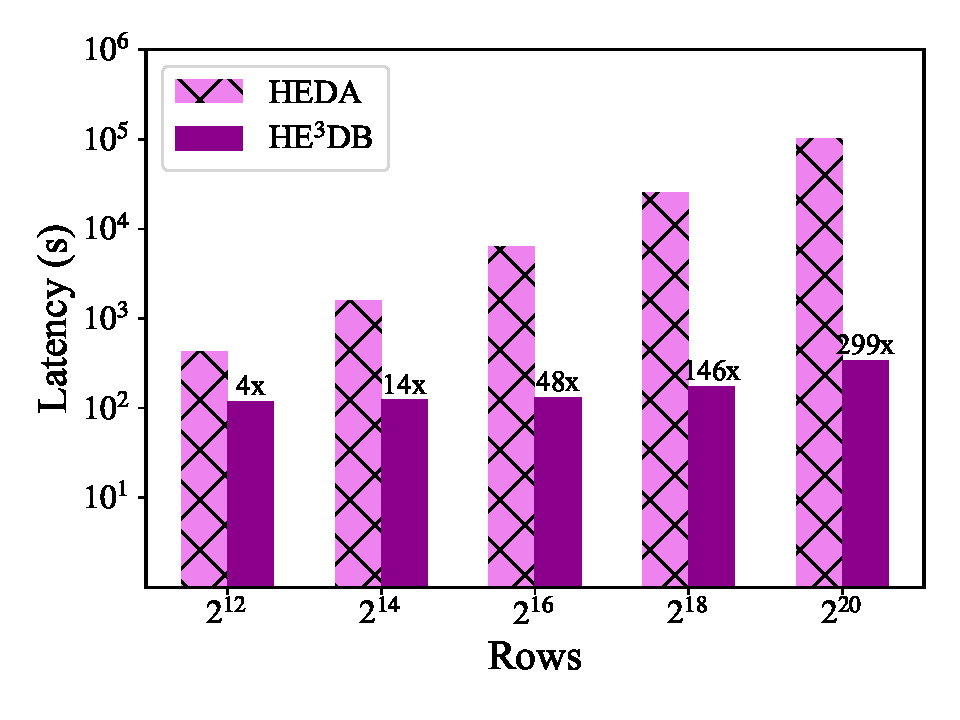
\includegraphics[width=\linewidth]{figure/compare_q1_heda.pdf}
    % \vspace{-1em}
    \caption{Query 1}
    \label{fig: hedaq1}
    \end{subfigure}%
    % \hfill
    \begin{subfigure}[b]{0.25\textwidth}
    \centering
    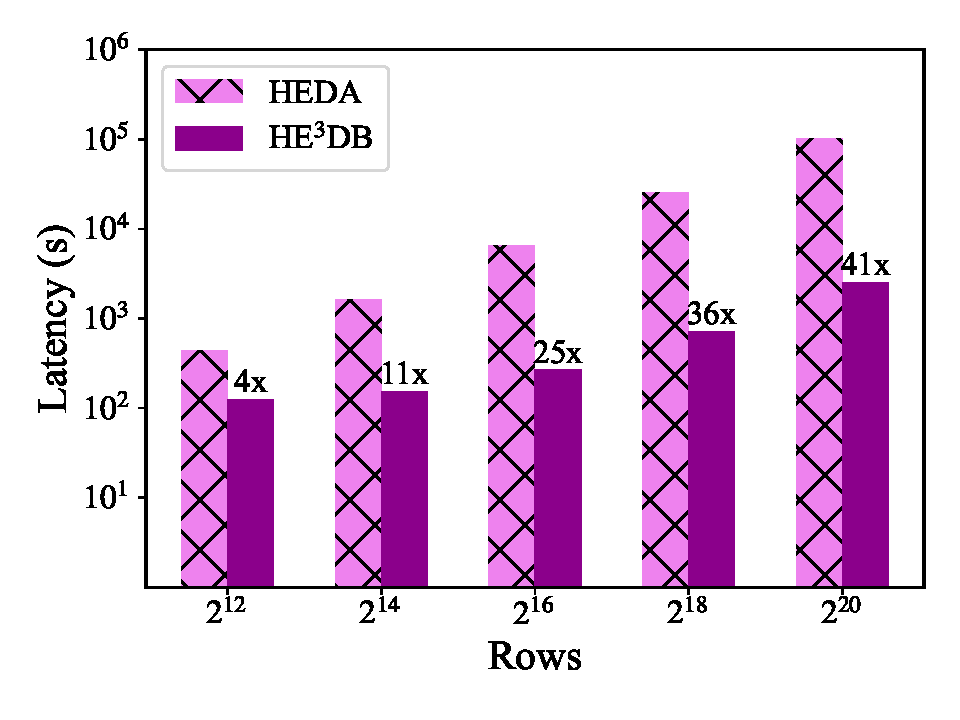
\includegraphics[width=\linewidth]{figure/compare_q6_heda.pdf}
    % \vspace{-1em}
    \caption{Query 6}
    \label{fig: heda16}
    \end{subfigure}%
    % \hfill
   \end{center}
    % \vspace{-1em}
      \caption{Comparison between \NAME and HEDA~\cite{sagma} on their modified TPC-H Query 1 and Query 6 with varying sizes of $\dbtabrow$.} 
      \Description{Comparison between \NAME and HEDA~\cite{sagma} on their modified TPC-H Query 1 and Query 6 with varying sizes of $\dbtabrow$.
      As the size of $\dbtabrows$ increases, 
      the advantage of our performance is more obvious.}
   \label{fig: hedabench}
   % \vspace{-0.5em}
\end{figure}

% {\bf{Aggregation Only}}:
%\paragraph{Aggreagation Only}


\begin{figure}[t!]
   \begin{center}
    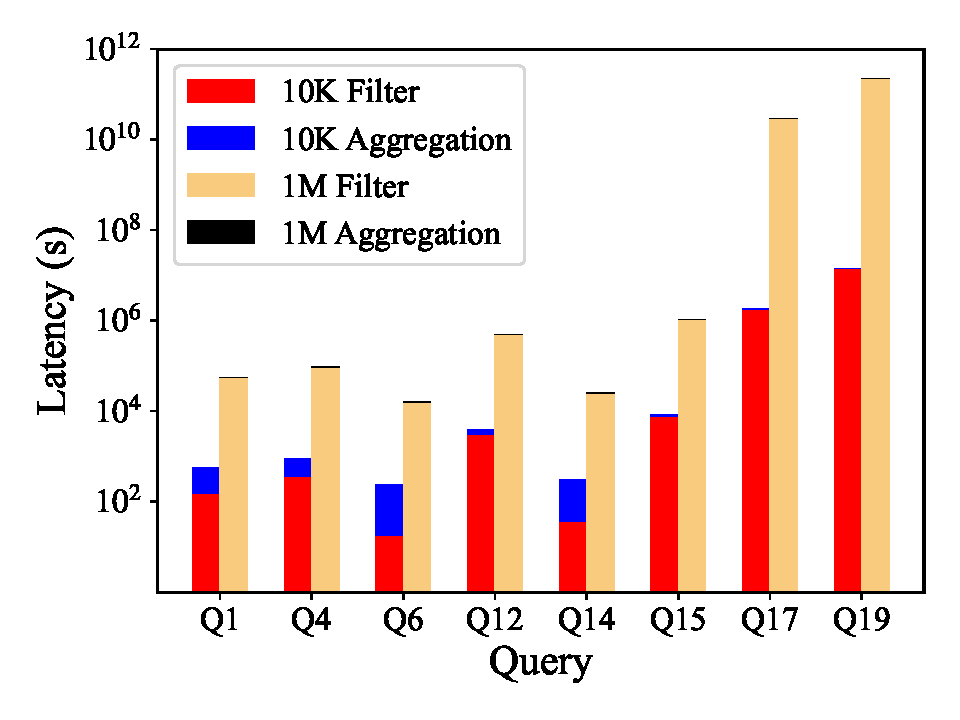
\includegraphics[width=0.9\linewidth]{figure/tpc_h.pdf}
   \end{center}
    % \vspace{-0.5em}
      \caption{Latency performance of \NAME on various TPC-H benchmark
      over different sizes of $\dbtabrow$.} 
      \Description{Latency performance of \NAME on various TPC-H benchmark
      over different sizes of $\dbtabrow$.
      As the size of the database increases, the bottleneck of the entire SQL lies in the filtering period.}
   \label{fig: tpchbench}
   % \vspace{-0.5em}
\end{figure}

% {\bf{TPC-H Benchmarks}}:
%\paragraph{TPC-H Benchmark}
We compare \NAME with HEDA, one of the most recent FHE-based encrypted DBMS
that supports unbounded-depth filter-aggregation~\cite{heda}. As shown in 
\cref{fig: hedabench}, on the same set of TPC-H queries, \NAME 
is on average $299\times$ faster on TPC-H Query 1 and $41\times$ faster on 
TPC-H Query 6. To closely examine the performance breakdown of \NAME,
we test a variety of the TPC-H benchmark queries on our \NAME framework, 
and the results are outlined in \cref{fig: tpchbench}. As the figure shows, while 
the filtering and aggregation latency are somewhat balanced on smaller databases,  
the filtering latency becomes the main performance bottleneck
as the size of the database gets larger. Overall, we can evaluate an end-to-end
SQL query over a 10K-row database within 241 seconds.

%\subsection{An End-to-End Decision Tree Benchmark}\label{eva:pdte}

% After query process, we use the function described in \cref{Analysis: Bridge} to bridge the gap between 
% aggregation result and data analysis. 
% {\bf{End-to-End Decision Tree Benchmark}}: 
%\paragraph{End-to-End Decision Tree Benchmark}
For the evaluation of the private decision tree, 
we provide a brief summary of the evaluation results obtained over
multiple decision tree models under a computation outsourcing setting, where both
the inputs and the model weights of the decision trees are ciphertexts.
% through our \pdte on 
% the experiment environment described \cref{eva:Arch}. 
To enable fair comparisons, we use the same datasets 
as in~\cite{sortinghat}, and reworked the implementation of~\cite{sortinghat} such that the
solution in~\cite{sortinghat} can also operate over encrypted inputs and model weights.
%\cref{fig: homtreebench} compares the performance of \NAME and \cite{sortinghat} on  
%end-to-end decision tree benchmark. 
While detailed comparison results can be found in the appendix, we achieve 12x--326x faster 
evaluation speed than~\cite{sortinghat} over a wide range of datasets and input sizes.
Thus, by adding the powerful online data analysis
capability to the expressive query evaluation framework,
\NAME is able to significantly improve the efficiency, usability
and practical applicability of outsourcing databases securely.
% able to significantly narrow
% the performance and usability gaps between theoretical FHE-based encrypted
% database constructions and practical needs for SDO in the real world.
% improve the 
% practicality of secure database outsourcing based on fully homomorphic encryption.

